% Created 2020-12-13 Sun 20:22
% Intended LaTeX compiler: pdflatex
\documentclass[11pt]{article}
\usepackage[utf8]{inputenc}
\usepackage[T1]{fontenc}
\usepackage{graphicx}
\usepackage{grffile}
\usepackage{longtable}
\usepackage{wrapfig}
\usepackage{rotating}
\usepackage[normalem]{ulem}
\usepackage{amsmath}
\usepackage{textcomp}
\usepackage{amssymb}
\usepackage{capt-of}
\usepackage{hyperref}
\usepackage[margin=0.8in]{geometry}
\usepackage{amssymb,amsmath}
\usepackage{graphicx}
\documentclass[12pt]{article}
\usepackage{hyperref}
\usepackage{multicol}
\usepackage[T1]{fontenc}
\usepackage[utf8]{inputenc}
\graphicspath{{.}}
\usepackage{cite}
\author{Andrea Malleo and Reggie Gomez}
\date{\today}
\title{Occupancy Networks: NYU Computer Vision Fall 2020 Final Project}
\hypersetup{
 pdfauthor={Andrea Malleo and Reggie Gomez},
 pdftitle={Occupancy Networks: NYU Computer Vision Fall 2020 Final Project},
 pdfkeywords={},
 pdfsubject={},
 pdfcreator={Emacs 26.3 (Org mode 9.4)}, 
 pdflang={English}}
\begin{document}

\maketitle
\section{Intro}

\begin{multicols}{2}
We present an implementation of an existing technique for 3D reconstruction by the learned approximation of the decision boundary of 3D objects. Specifically we followed the method presented in Occupancy Networks [citation] to train a neural network classifier to learn the continuous decision boundary representing the implicit surface of some class of objects for the generation of 3d meshes. The model can then map any coordiante in 3d space to either a 0 or 1, indicating whether that point lies outside of inside of a mesh respectively. This generation (inference) process is both conditioned on still images of the desired category and unconditioned, decoding from a learned latent variable representation to produce a continuous distribution of instances of a category.
\par
\\
A learned model for 3D representation sits a layer above existing methods for storing 3D representations such as point clouds, voxels, and meshes, in that the model can generate countless instances of all three. The trained Occupancy Network evaluates at any point whether or not that point lies within a mesh. It can be evaluated on a grid of points of arbitrary resolution and exhibits generative capabilities on an entire category of objects. From these coordinates and their occupancies values, point clouds can be extracted directly, namely by taking all of the coordinates with an occupancy value of one. For the actual mesh representation, further computation is necessary. Specifically, inputting the output of the model into the Marching Cubes algorithms will produce meshes such as the one in [citation Figure 1]
\par
\\
The Occupancy Networks [citation] paper came out as one of a small batch of papers in 2019 all showcasing similar work learning implicit fields for generative shape modeling. In [citation] not just a binary classification but a learned continuous signed distance function is used to generate a class of shapes by evaluating the magnitude of distance and the classification (negative inside/positive outside) at any point relative to the surface boundary. On the generative side, OccupancyNetworks [Citation], and us in their footsteps, use a variational auto-encoder to learn the mean and standard deviation of Gaussian distribution on a 128 dimension latent vector representing instances of a mesh in some class, whereas [citation] formulates their own auto-decoder that sidesteps the need for an encoder component in the model architecture. Deep Level Sets [citation] and Learning Implicit Fields for Generative [citation] also present networks that produce inferred 3D shapes exhibiting smoothness, continuity, and detail not found in their recent forerunners.

%\begin{wrapfigure}{r}{0.25\textwidth}
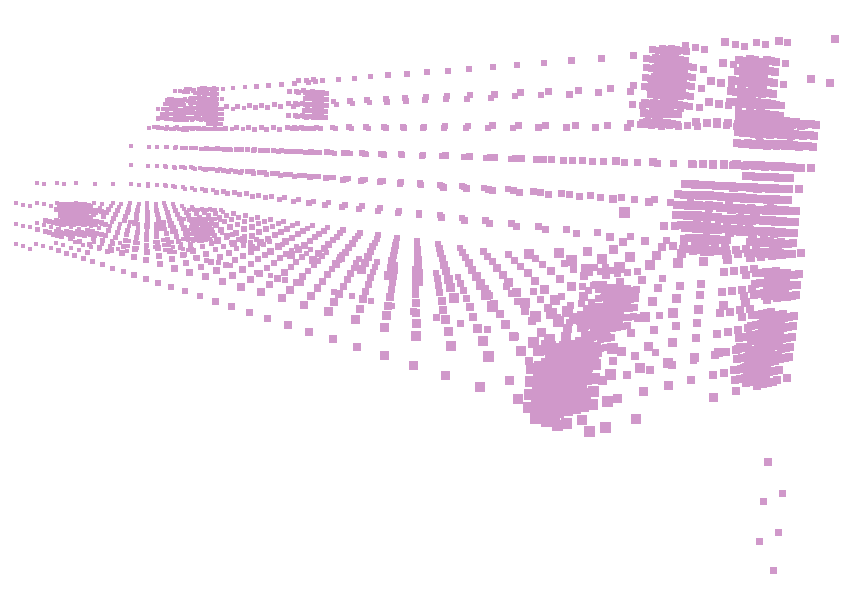
\includegraphics[scale=0.3]{benchImages/bench_pointcloud.png}
%\centering
%\end{wrapfigure}

\section{Method}
In this section we discuss the source and preprocessing of the training data. Then we outline the goals of the three experiments we conducted and compare and contrast the model architectures and training times. Finally we touch on the inference process, and the follow up steps for visualizing the resultant meshes.


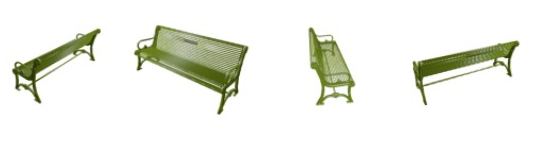
\includegraphics[scale=0.75]{sampleTrainingBench/benches.png}

 The dataset used to train all the models was downloaded preprocessed from the authors of Occupancy Network [citation]. The data is from the ShapeNet [citation] dataset and for each category of shapes (chair, bench, cabinet, sofa) there are thirteen still images of an instance of that object, taken from different orientations. See Figure 2[citation]. Additionally, for each instance, there are 100,000 coordinates from uniform sampling of the unit cube centered at (0,0,0). For each of points there is a corresponding ground truth occupancy value in $\{0,1\}$. The preprocessing steps that we did not repeat include filtering out non-water tight meshes from the original dataset, and running the algorithm that determines this ground truth. \\




\subsection{Training}
All model architectures [citation (GITHUB)] emulate those used in the paper [citation]. Where any component was unclear from the description and images of the paper, we consulted the available implementation [citation]. All three experiments share the same main architecture and differ in their means of computing an encoding on which to condition the training, either from a 2d image tensor, or from the points themselves.
\par
\\
Experiment one concerns the generation of meshes conditioned on a still image of an instance of the input category.  The input to each 'mini-batch' consisted of a single image of a image, randomly drawn from the thirteen available for each instance and some $K$ coordinate points from the ground truth of that mesh. The image went into an encoder block, which in this case was a downloaded ResNet-18 architecture pretrained on the ImageNet dataset \hyperlink{ref5}{5}. That output is passed into a fully-connected layer to project the features to a 256 dimension encoding $c$. The points meanwhile are essentially passed through five ResNet [citation] blocks. Crucially, the conditional batch normalization
\begin{flalign*}
  x_{out} = \gamma(c)b + \Beta(c)\\
\end{flalign} is computed twice inside of each ResNet block where
\begin{flalign*}
  b &= \frac{x_{in}-\mu}{\sqrt(\sigma^2 + \epsilon)}\\
\end{flalign*}
is the BatchNorm1d with affine set to False and track running stats set to true.
Note that each time conditional batch normalization is performed, $c$, computed once, is passed through two disjoint fully connected layer heads to generate the backprop refined $\Beta$ and $\gamma$ vectors. The loss function used during training is cross entropy classification loss averaged over all points across all minibatches. Let $B$ denote the batch size and $K$ the number of points for each instance or minibatch.
\begin{flalign*}
  L(\theta, \psi) &= \frac{1}{B*K} \sum_{i=1}^{B} \sum_{k=1}^K L(f_{\theta}((p_{ij},z_{ij}),o_{ij}))
\end{flalign}
\\
\par
Experiment three involved learning a probabilistic latent variable model for representing the mesh function space. This model just takes points and occupancies, and first passes the points in to the encoder module. This encoder module is a slight variation on the Point Cloud Completion encoder just described, the most significant difference being that the output are two vectors for the mean $\mu_{\psi}$ and log-standard deviation $\sigma_{\psi}^2$ of the 128 dimensional latent code z. In the forward pass, once these two vectors are computed, a sample from this distribution is drawn as $(e^{\sigma}*rand()+ \mu)}$. This 128 dimensional vector is now used just as the encoding used just as in experiment one for the conditional batch normalization. The loss function here is two pronged, composed of both the binary cross entropy loss between the computed probablities and the targets, and the KL divergence of the generated $\mu_{\psi}$ and $\sigma_{\psi}$ from a Gaussian distribution of mean 0 and standard deviation 1. [citation] \begin{flalign*}
    L(\theta, \psi) &= \frac{1}{|B|} \sum_{i=1}^{|B|} \sum_{k=1}^K L(f_{\theta}((p_{ij},z_{ij}),o_{ij})) \\
    &+  \frac{-1}{2} \sum (1 + \sigma_{\psi} - \mu^2 - e^{\sigma_{\psi}} )
\end{flalign}

\subsection{Mesh Generation}
The mesh generation procedure can be summarized as follows. The trained model takes a batch of coordinates in 3d space and either a single still image to condition the output (experiment 1), or a random variable drawn from the learned distribution (experiment 2). The first step of inference would be to generate a set of coordinates that uniformly sample the 3d unit cube centered at (0,0,0). Because the network learns a continuous occupancy function, it can be evaluated at any resolution. One of the drawbacks of existing 3D representations is the cubic memory demand of voxels. This can be mitigated by what the Occupancy Network authors termed \textbf{Multiresolution IsoSurface Extraction}. Namely, we began by evaluating the occupancy on a $32x32x32$ grid of voxels. The output of the model is the probability that this point lies within the mesh. We set a threshold value of 0.1 in experiment 1, and 0.3 in experiment 2, at or above which a point is given an occupancy value of 1, otherwise it is marked 0. Next for every voxel whose corner coordinates are a mix of occupied and unoccupied, this cube is divided into 8 subvoxels and reevaluated at all of its points. This process is repeated at most one more time, for a recursion depth of 2. In practice we have a grid that adapts to a finer grain resolution at the boundary of the mesh to allow for a more precise estimation of edges, not wasting memory by storing more than a coarse grid around the exterior of the mesh.
\par
\\
Once we have a suitable set of coordinates written to one file, and their cooresponding occupancy values written to another, the next step is to apply the Marching Cubes algorithm [citation] to generate a set of triangles that compose the mesh. The Marching Cubes algorithm iterates over each voxel cube and considers the occupancy values at each corner. For each of the 256 permutations of possible patterns of occupancy (occupies or does not occupy for each of the 8 vertices), there are only about 15 unique cases (in the original publication). These are all tabulated in a map, and correspond to the set of triangles inferred from the estimated points of intersection. The union of all of the triangles found defines the mesh.
\\
\par
The .off files written by Marching Cubes can be visualized most simply with a 3rd party opensource application such as Meshlab. We did however input these mesh files into a rasterizer written as part of the Computer Graphics class this semester and generated stills and gifs of the resultant meshes. Please go to our github page to see gifs. For experiment 1, please see the video that rotates around the generated bench mesh. For experiment 2, please see the video that illustrates interpolation in latent variable space, and the resulting continuous deformations to the couch mesh.

\end{multicols}

\section{Experiments}

\textbf{Experiment 1:} The goal of the first experiment was to train a model that achieves 3D mesh reconstruction from a single 2D image of the object from an arbitrary angle of view. In our case we trained on the bench category.

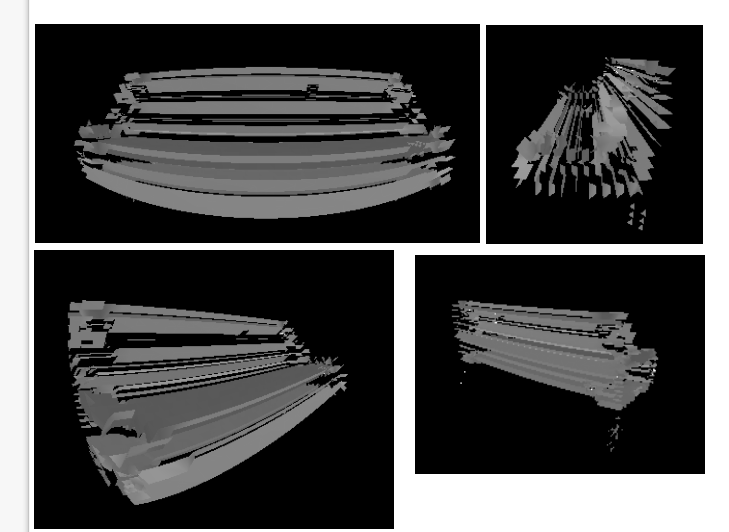
\includegraphics[scale=0.75]{./benchImages/benches.png}

\textbf{Experiment 2:} The goal of the second experiment was to learn a distribution over a latent embedding of the mesh category for unconditioned generation of 3d meshes and demonstrate the continuous nature of this distribution by interpolating in the latent space.

\section{Discussion}


\section{References}
  \begin{enumerate*}
    \item \hypertarget{ref1}{[1]}  Lars and Oechsle, Michael and Niemeyer, Michael and Nowozin, Sebastian and Geiger, Andreas. Occupancy Networks: Learning 3D Reconstruction in Function Space Mescheder, In Proc IEEE Conf. on Computer Vision and Pattern Recognition (CVPR).2019
    \item \hypertarget{}{[]} https://github.com/autonomousvision/occupancy\_networks
    \item \hypertarget{ref5}{[5]} J. Deng, W. Dong, R. Socher, L. jia Li, K. Li, and L. Fei-fei.  Imagenet:  A large-scale hierarchical image database.  InProc. IEEEConf. on Computer Vision and Pattern Recognition (CVPR), 2009.
    \item \hypertarget{}{[]} Jeong Joon Park and Peter Florence and Julian Straub and Richard Newcombe and Steven Lovegrove. DeepSDF: Learning Continuous Signed Distance Functions for Shape Representation. arXiv:1901.05103. 2019
    \item \hypertarget{}{[]} Mateusz Michalkiewicz and Jhony K. Pontes and Dominic Jack and Mahsa Baktashmotlagh and Anders Eriksson. Deep Level Sets: Implicit Surface Representations for 3D Shape Inference. arXiv:1901.06802. 2019
    \item \hypertarget{}{[]} Zhiqin Chen and Hao Zhang. Learning Implicit Fields for Generative Shape Modeling. arXiv:1812.02822. 2019.

  \end{enumerate}
\end{document}
